\chapter{Activos financieros en los que invertir}


\section{Activos Financieros}

Los activos financieros son los productos que vamos a comprar o vender.

¿Cuáles son los más importantes?:
\begin{itemize}
    \item Acciones.
    \item Bonos.
    \item Divisas y 
    \item Derivados financieros.
\end{itemize}
No son los únicos, pero sí los más negociados en el mercando y en los que nos centraremos.

\subsection{Acciones}


Los activos financieros más conocidos son las \ti{acciones}, pero ¿qué son las acciones? y ¿cómo podemos ganar dinero invirtiendo en ellas?. Por ejemplo, las empresas cuando necesitan financiar su crecimiento, una de las opciones que tienen para obtener fondos del exterior es mediante la emisión de acciones. El \ti{accionista} es quien compra las acciones, convirtiéndose en un \ti{pequeño propietario de la empresa} con una serie de derechos, de los cuales, el que más nos interesa es el \tb{derecho a recibir dividendos}. Los dividendos se producen cuando la empresa tienen beneficios y los reparte entre los accionistas. Por lo tanto, a la hora de invertir nos interesa conocer los dividendos.

No sólo existe esa forma de obtener rentabilidad de la compra de las acciones, también podemos obtener rentabilidad a partir de la \tb{revalorización de las acciones}, es decir, compramos a un precio y las vendemos en el futuro a un precio mayor. 

En función de cuál será nuestro \ti{perfil inversor}, daremos más peso al \ti{análisis de los dividendos} o al de la \ti{revalorización} y, en función de nuestro perfil (inversor a largo o corto plazo), diseñaremos unas estrategias para ver en qué acciones invertiremos.

Junto con las acciones, tenemos la opción de invertir en \tb{índices}, como son:
\begin{itemize}
    \item Dow Jons
    \item SP\&500 
    \item NASDAQ
    \item IBEX-35
    \item EURO-STOCK-50,\ldots
\end{itemize}

Los \ti{índices \tb{no son acciones}}, lo que persiguen es explicarnos cuál es el momento general del mercado, si sube o baja, no sólo viendo una acción sino el conjunto de aquellas acciones que son las más importantes. Normalmente se seleccionan aquellas empresas que tienen una mayor capitalización, que son más grandes y que tienen mayor liquidez en el mercado. Todos los mercados, a nivel internacional, tienen su índice de referencia.

Invertir en índices tiene la ventaja, frente a invertir en acciones individuales, que a largo plazo presentan una tendencia alcista y nos permiten diversificar, ya que los índices están compuestos por diferentes acciones de diferentes sectores, con lo que tenemos menor riesgo que si compramos acciones de una única empresa, evidentemente es una buena opción para invetir a largo plazo.

¿Qué hacemos si queremos seguir en un índice?¿cómo podemos invertir de forma que si el índice sube obtengamos una rentabilidad positiva?. Hasta hace poco, la opción era hacer:
\begin{itemize}
    \item \tb{réplica total}, cuando compro todas y cada una de las acciones que componen el índice, en la imagen vemos los componentes del Dow Jones 30, tendríamos que comprar todas esas acciones en la misma proporción en las que están en el índice.
    \begin{center}
        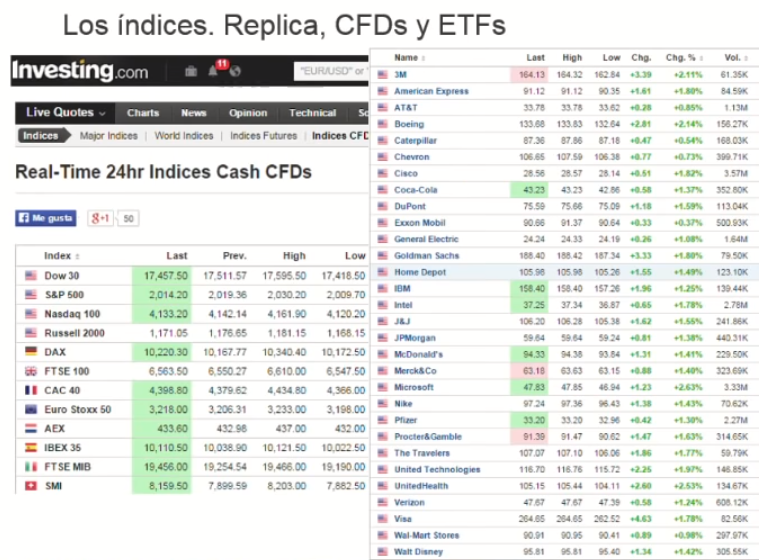
\includegraphics[scale=.65]{images/mod04_01.png}
    \end{center}
    En este caso, las empresas están equiponderadas, cada una tiene una \ti{treintava parte del peso del índice}, esto supondría comprar treinta acciones que nos generaría una serie de gastos y comisiones de depósitos. 
    \item \tb{réplica parcial}, mediante el uso de modelos matemáticos se seleccionan unas cuantas empresas del índice, le damos un peso en nuestro propio índice, nuestra réplica, y obtendremos una rentabilidad similar a la que obtiene el índice de referencia, de esta manera pues ahorramos costes.
\end{itemize}

Estas eras las opciones únicas que había hasta hace poco, ahora también podemos invertir en las opciones más comunes, las más populares como son 
\begin{itemize}
    \item \tb{CFDs (Contracts for Difference)}, son contratos que el inversor y una entidad financiera acuerdan intercambiarse, la diferencia entre el precio de compra y el precio de venta de un determinado activo subyacente. Pueden ser un valor negociable: índices, divisas, tipos de interés y otras activos de naturaleza financiera.
    \item \tb{ETFs (Exchange Traded Funds)}, son fondos cotizados; su principal función es replicar un determinado mercado e intetar ofrecer el mismo rendimiento. Existen fondos sobre renta fija, renta variable, divisas y materias primas. Son una mezcla entre fondo de inversión y acciones.
\end{itemize}

Se pueden comprar y vender como si fueran acciones, pero al ser también instrumentos derivados tienen una problemática adicional.


\subsection{Bonos}

Son emisiones de renta fija que también emplean las empresas para financiar su crecimiento. Las empresas, no sólo emiten acciones sino que lo que realmente financia su crecimiento son las emisiones de renta fija.

La \tb{renta fija} es el mecanismo de una empresa para captar dinero, crea un bono u obligación y la vende en el mercado, aquellos que compran ese bono tienen derecho a que la empresa les devuelva el dinero más unos interses, con lo cual se puede saber con anterioridad cuales van a ser los flujos de caja qué dinero nos va a generar el haber comprado ese bono, por eso es renta fija frente a las acciones que son renta variable.

Los tipos de bonos son:
\begin{itemize}
    \item las \tb{letras} y los \tb{pagarés}, que son a corto plazo,
    \item los \tb{bonos}, a medio plazo, y 
    \item las \tb{obligaciones}, a largo plazo. Existen obligaciones que son \ti{perpetuas}, no vencen nunca.
\end{itemize}

¿Cómo se obtiene rentabilidad comprando renta fija? Mediante los intereses que deben pagar por haber comprado el bono pero, además, tenemos la posibilidad de la revalorización del bono. Los bonos una vez se emiten en el mercado primario, se pueden negociar en el mercado secundario igual que ocurre con las acciones, por esta razón su precio dependerá de la oferta y la demanda, es decir, el precio de un bono puede subir y puede bajar. Es importante tener esto en cuenta, porque mucha gente cree que al invertir en renta fija no puede perder dinero, no es el caso si tengo un bono, lo compro y lo mantengo hasta el vencimiento yo sé cuál va a ser la rentabilidad, pero si compro o vendo en el mercado secundario, ahí puedo ganar más dinero, pero también perderlo; por lo tanto, si nos dedicamos a invertir en bonos también se pueden diseñar estrategias de inversión, para comprar bonos a precio barato y venderlos a un precio más elevado.

¿De qué depende que un bono suba o baje de valor en el mercado secundario? De la oferta y demanda y de las expectativas de la evolución, que dependen a su vez de factores macroeconómicos, políticos y que está relacionado sobre todo con la evolución de los tipos de interés, con el riesgo de crédito.

En los bonos no son sólo las empresas quienes los emiten, también tienen un peso específico muy grande los estados.

\subsection{Divisas y derivados financieros}

\subsubsection{Divisas}

Las \tb{divisas} son los medios de pago de curso legal en los distintos paises y en los mercados financieros internacionales. Los que más se negocian son el dólar americano, el euro, el yen japonés y la libra esterlina, pero existen otras. Hay que tener en cuenta que \ti{no todas las divisas son convertibles}. Inicialmente, las divisas se compraban y vendían para adquirir bienes y servicios en países extranjeros, hoy en día no tienen nada que ver con las transacciones en la economía real, sino que se deben principalmente a las operaciones en los mercados financieros, también soportan un elevado porcentaje de especulación.

El \ti{mercado de divisas no es un mercado organizado}, ésto significa que si quiereo comprar acciones de una empresa, INDITEX o Microsoft, voy al mercado organizado y puedo comprar  a un precio concreto, en el caso de las divisas no existe un único mercado, sino que hay muchos con tipos de cambio diferentes para la misma divisa. Es importante, que al operar con divisas cuidemos con qué broker, o dealer, vamos a operar para tener un tipo de cambio y comisiones ventajosas, y además fijarse en el \ti{riesgo de crédito}, tener en consideración que el broker quiebre, es un factor muy importante, que no se suele tener en cuenta, pero que no es infrecuente.

¿Qué variables influyen el tipo de cambio de las divisas?. En divisas la estrategia es \ti{comprar barato} y \ti{vender caro}:
\begin{itemize}
    \item Oferta y demanda
    \item Expectativas, factores políticos y macroeconómicos:
    \begin{itemize}
        \item inflación
        \item tipos de interés
        \item política fiscal
        \item balanza de pagos, etc.
    \end{itemize}
\end{itemize}
al margen de estas variables, análisis económico, tenemos la opción de invertir utilizando estrategias de análisis técnico, que también ofrecen buenos resultados y son las que hay qu seguir en la inversión a corto plazo.

\subsubsection{Derivados financieros}

Los derivados financieros, cada uno tiene características diferentes, en cuanto al propio producto, cómo se negocia, en qué tipo de mercado,\ldots 

Algunos de los derivados financieros más conocidos son:
\begin{itemize}
    \item Futuros
    \item Opciones
    \item Warrants
    \item Swaps
    \item Fras 
    \item CFDs,\ldots
\end{itemize}

Hay que tener en cuenta que cuando hay un derivado siempre existe un activo subyacente. El derivado es un \ti{producto sintético} que se crea en base a un activo subyacente, un activo real que también cotiza como son: acciones, índices, tipos de interés, materias primas, precios de la energía, \ldots

La idea es que el derivado tenga un comportamiento similar en el precio al activo subyacente. Además tienen una serie de características intersantes para nosotros al invertir:
\begin{enumerate}
    \item Permiten ganar dinero en mercados alcistas o bajistas. El mecanísmo es que nosotros tenemos el concepto de compramos una acción y luego se vende, con los derivados esto no es así, para cerrar la posición tengo que comprar y vender o vender y comprar.
    \item No es necesario adquirir el activo subyacente. Puedo especular con el precio del petroleo, pero no es necesario que compre un barril brent o texas, nos permite seguir la evolución de un activo sin adquirir realmente el activo.
    \item En la mayoría de los derivados, las plusvalías y minusvalías se liquidan diariamente. Esto es importante ya que si el derivado baja tenemos que pagar las pérdidas potenciales, minusvalías, es importante porque puedo quedarme sin dinero conforme el derivado vaya bajando de precio. 
    \item Además, para trabajar con derivados se suelen exigir garantías que hay que tener depositadas, y cuando esas garantías se consumen, porque se ha perdido todo ese dinero, la posición se cierra, cuando es posible, ya que puede que haya pérdido más dinero del depositado como garantía, con lo que tendría que aportar el dinero adicional.
    \item Alto grado de apalancamiento, implica que con poco dinero desembolsado, el dinero de las garantías,  puedo obtener una rentabilidad muy elevada. Pero hay que tener en cuenta que la rentabilidad puede ser positiva y negativa.
\end{enumerate}